\documentclass{article}
\usepackage[english]{babel}
\usepackage[letterpaper,top=2cm,bottom=2cm,left=3cm,right=3cm,marginparwidth=1.75cm]{geometry}
% Useful packages
\usepackage{amsmath}
\usepackage{graphicx}
\usepackage{adjustbox}
\graphicspath{ {/home/hal9000/code/ConvectionDiffusionMsolve/ResultsReport/Dynamic3DResultsReport/images/} }
\usepackage{float}
\usepackage[colorlinks=true, allcolors=blue]{hyperref}



\title{Bigg Mann$++$ Documentation}
\author{Ch. Orestis Papas}


\begin{document}
	
	\section{Abstract}
	This report presents the development and implementation of BiggMann++, an object-oriented C++ software specifically designed to solve second order partial differential equations (PDEs) in their most generalized form. The extensive utility of the software extends across numerous fields and disciplines, highlighting the universal presence of second order PDEs in a wide array of scientific phenomena. BiggMann++ embodies the developer's perspective on the physical world, the transition from continuum to discrete, from the beautiful mathematical symbols to computer memory pointers, and encapsulates a shift towards a more abstract interpretation of engineering problems. This perspective acknowledges that beneath the myriad physical phenomena and their varied coefficient nomenclatures reside identical core mathematical structures.
	
	BiggMann++ was originally devised as a $C\#$ project for the "Mesh Generation" course during my master's program, with its primary focus being the generation of structured node grids by solving elliptic PDEs in parametric space. As the software evolved, so did my perspective, particularly during my research in the area of tumor development modeling. An insightful observation dawned upon me: the core mathematical constructs remained essentially unchanged, regardless of whether the coefficient represented the oxygen diffusivity in an oxygen mass transport equation, the $g_{ij}$ component of the contravariant tensor in mesh generation. This epiphany underscored the universality of second order PDEs, revealing their beauty and pervasive presence across diverse scientific disciplines. Recognizing this pattern was a significant shift in perspective and ultimately inspired the transformation of BiggMann++ into a more generalized and parametrized tool for that offers control over the complete simulation process. The framework has transitioned to C++ over the course of the last 6 after the need for custom memory management emerged. It allows user friendly manipulation of every aspect of the simulation from computational domain definition and mesh metrics to node and direction dependent PDE coefficients. Performance is also considered, but 
	

	
	\section{Software Framework}
	\subsection{Core Development Principles}
	The primary objective of this development effort was to construct a codebase that is easy to understand, readable, and indicative of the thought process embedded in its creation. The code employs terms familiar to any engineer for clarity. The adoption of object-oriented principles was an essential strategy to boost maintainability and circumvent error susceptibility, specifically by avoiding code repetition and casuistry. The key concepts are presented below:
	
	
	\begin{itemize}
		
		\item Complete Avoidance of External Libraries: The only non-custom utility used is the standard library. All numerical methods such as matrix-matrix and matrix-vector multiplication, as well as matrix decomposition, are based on the custom $std::vector<T>$ container class \texttt{Array<T>}. This approach improves understanding and control of the data structures used and leads to a better understanding of C++.
		
		\item Descriptive Naming and Avoidance of "Master Classes": Each variable, function, and class is named in a highly readable and explanatory manner. Classes are organized in such a way that their actions align with user intuition.

		
		\item Space Description: The computational space where the PDE is applied, and the relative positioning of two random points, is described with enumerations (enums).
		
		\begin{itemize}
			\item Coordinate System: enum Direction (One, Two, Three, Time, None) \newline
			This encapsulates any coordinate system that can be described using three orthonormal axes (1,2,3).
			
			\item Relative Positions: enum Position (TopLeft, Top, TopRight, Left, Center,...,LeftTopBack). \newline
			The consistent identification of nodes, combined with the properties of the isoparametric curves of the mesh, leads to an intuitive and robust description of the relation between any nodes with $O(1)$ complexity for all three Directions.
			
			\item Coordinates: enum CoordinateType (Natural, Parametric, Template). \newline
			This provides information about the spatial representation of each node, aiding in the calculation of mesh metrics.
		\end{itemize}
		
		\item Schemes for Uniform and Non-uniform Node Distribution: The program exhibits the versatility to compute both the textbook, hardcoded Finite Difference (FD) schemes with errors of order $O(\Delta x^6)$ for uniformly distributed nodes, and scheme weight for nodes distributed in an arbitrary manner, maintaining an error order of $O(\Delta x^n)$.
		
		\item Consistent Cut-off Error Scheme: To apply a scheme with consistent accuracy across the entire domain, Finite Difference Schemes of different types (Forward, Backward, Central) and the same accuracy are applied according to the number of available neighbors. The algorithm successfully determines the graph of each node without considering special cases, leading to accurate higher order schemes.
		
		\item Space Decomposition: The implementation of enums and maps allows for the decomposition of the domain into Directions. The contribution of each Direction in all parts of the analysis is treated in loops without taking special cases under consideration.
		\end{itemize}
	\subsection{Generalized Second Order Partial Differential Equation}


	\noindent In the current development state the user can solve the following equations in 2D with Dirichlet Boundary Conditions
		\begin{itemize}
			\item Laplace Equation
			\item Poisson Equation
			\item Steady State Transfer of any scalar or vector $\phi$ via the Convection-Diffusion-Reaction Equation
		\end{itemize}

		
	\section{Framework Description}
	The program aims to provide a complete simulation package for the user. It starts with an analysis that solves the Poisson equation for the structured grid creation, then proceeds to the actual engineering application. The underlying mechanisms for each analysis type are exactly the same.	

	\begin{figure}[H]

		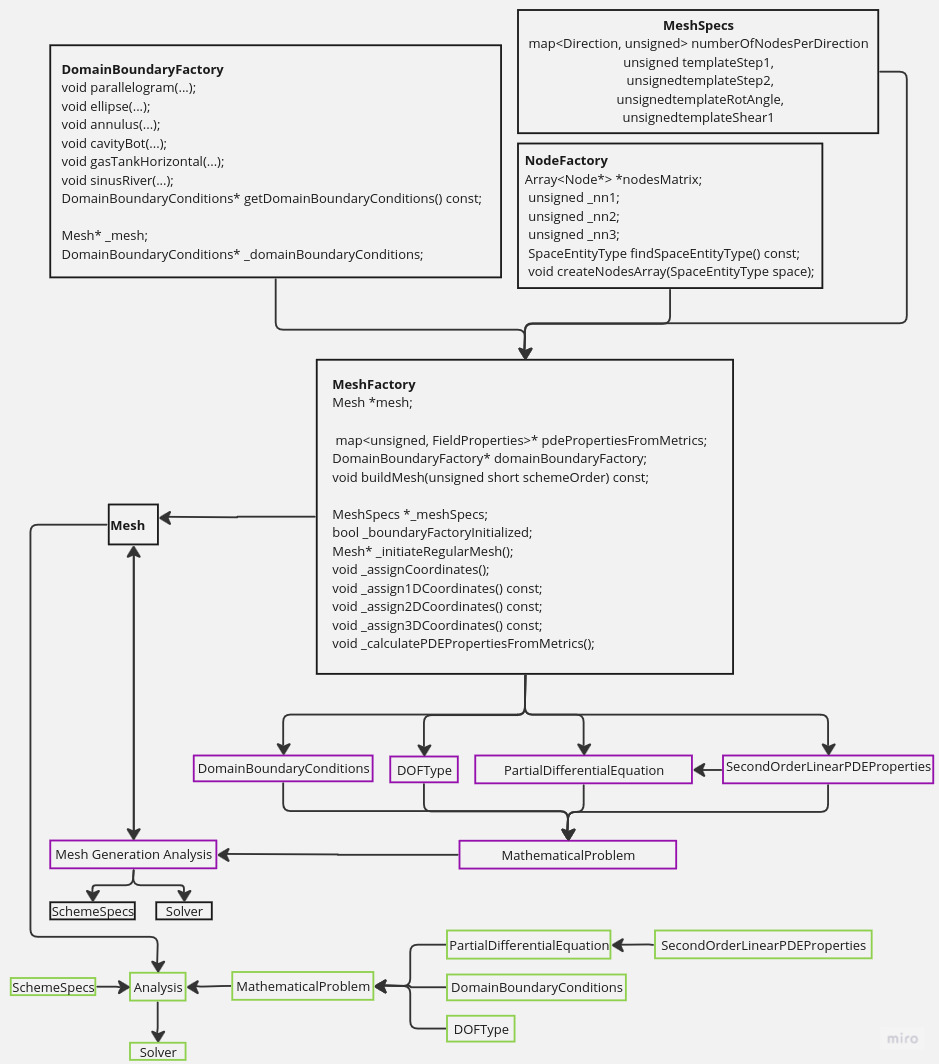
\includegraphics[height=1.0\textheight, width=1.05\textwidth, keepaspectratio]{./images/uml.jpg}
		\caption{UML Diagram of the BigMann analysis workflow. Green and purple frames correspond to the mesh generation and the physics simulation components correspondingly}
		\label{fig:UML}
	\end{figure}
	
	\newpage
	
	\subsection {Numerical Analysis}
	
	The entire framework is built around the concept that a numerical analysis consists of a well-defined mathematical problem, a computational domain, and a solver. The mathematical problem comprises a Second Order Linear Partial Differential Equation with its corresponding coefficients, Degrees of Freedom, and Boundary Conditions. The coefficients and degrees of freedom define the scientific domain of the analysis.

	\subsection{Mathematical Problem}
	
	\subsubsection{Mathematical Problem - PDE and PDE Properties}
	The PDE is mostly defined by its coefficients. The user can choose between isotropic and anisotropic properties that apply in the whole domain or vary for each node. For a scalar or vector function $\phi = \phi(x_1, x_2, x_3,t)$ the general second order PDE takes the form:	$\boldsymbol{A} = Aij$ : 
	
	
	
	\begin{itemize}
		\item $A_{ij}$ for $i,j<3$ are the coefficients of the second order partial derivatives at each space direction. 
		
		\begin{itemize}
			\item When $A_{11}=A_{22}=A_{33}$ and $A_{ij}=A_{ji}$ the host medium is considered as isotropic meaning that it is symmetrical and homogeneous and has the same physical properties in all directions and it does not have any preferred direction of orientation. Examples of isotropic materials include most liquids and gases, as well as some solids such as glass and certain types of metals.
			
			\item When $A_{11} \neq A_{22} \neq A_{33}$ and $A_{ij}\neq A_{ji}$ the host medium is  anisotropic meaning that it is non-symmetrical and non-homogeneous. It does not have the same physical properties in all directions and it has preferred directions of orientation. Examples of anisotropic materials some metals and ceramics
		\end{itemize}
		
		\item $A_{i4},A_{4j}$ are the coefficients of the second order partial derivatives with respect to time.
		\begin{itemize}
			\item When $A_{i4},A_{4j} \neq 0$ the equation is transient. 
			\item When $A_{i4},A_{4j} = 0$ the equation is in steady state. 
		\end{itemize}
	\end{itemize}
	
	\subsubsection{Mathematical Problem - Boundary Conditions}
	Boundary conditions are defined using the Position enums, $std::map$, and lambda functions. The user can impose boundary conditions in the following ways:
	\begin{itemize}
		\item By setting a constant value across the boundary.
		\item By using a user-defined function of the boundary nodes coordinates $f(x_b, y_b)$.
		\item By assigning a different value at each boundary node.
	\end{itemize}
	At the time of writing, only Dirichlet Boundary Conditions are applied, but the implementation of Neumann conditions with improved accuracy is under development.
	
	\subsubsection{Mathematical Problem - Degree Of Freedom Types}
	The nature of the degrees of freedom in the framework are defined by the DOFType enum, and they are categorized in the DegreesOfFreedom vector field of the \texttt{Field\_DOFType} struct. For example, the DOF vector for the structured mesh generation problem is $\{Position1, Position2\}$.
	
	\subsection{Analysis Degrees of Freedom}
	The \texttt{DegreeOfFreedom} class embodies the essential attributes and functions related to degrees of freedom (DOFs) in the computational problem. This class provides the basic functionality to manipulate these DOFs, such as setting the value and retrieving the constraint type or parent node ID. It also provides comparison operators to compare two DOF instances.
	The Degrees of Freedom are applied on the mesh nodes. They are described by the following properties:
	\begin{itemize}
		
		\item \texttt{DOFType} : Enum describing tha type of the dof (Position1, Displacement2, Velocity3, Temperature, UnknownScalarVariable, UnknownVectorFieldVariableComponent1 etc.
		
		\item \texttt{ConstraintType} : Enum defyining whether a dof is Fixed or Free
		
		\item \texttt{id} : unsigned ID based on the Constraint Type. DOF ordering complies with nodal ordering (Left to Right, Bottom to Top, Back To Front) for both Fixed and Free DOFs.
		
		\item \texttt{value} : double that is initialized with NaN for Free dof and the boundary condition value for Fixed (Dirichlet) dof.
		
		\item \texttt{parentNode} :  unsigned that corelates the dof with the host Node ID.
	\end{itemize}
	
	The \texttt{DOFInitializer} class is responsible for the initialization of the DOFs for all the nodes in the mesh. The class constructor takes a mesh object, domain boundary conditions, and a list of DOFs types to be initialized. Depending on the nature of the boundary conditions (homogeneous or non-homogeneous), the initializer assigns fixed or free DOFs to the boundary nodes. Dirichlet and Neumann dofs are taged as Fixed or Free correspondingly, while all the internal dofs are Free. The class also provides functionality to assign unique IDs to each DOF depending on the \texttt{ConstraintType}, construct total DOF lists, and create additional data structures for efficient access to DOFs information.
	
	Finally, the \texttt{AnalysisDegreesOfFreedom} class leverages the functionality of the \texttt{DOFInitializer} to generate and store DOFs for a numerical analysis. This class maintains different vectors and maps to hold free, fixed, flux, and total DOFs for the analysis. It also records the count of different types of DOFs. The class destructor is responsible for the deallocation of the generated DOFs, ensuring that the memory management is handled effectively.	
	
	\subsection{Nodes}
	
	The \texttt{Node} class encapsulates the fundamental attributes and behaviors associated with a node in a discretized domain. It contains the following properties:
	\begin{itemize}
		\item \texttt{ID} : Unique Global ID
		
		\item \texttt{NodalCoordinates} : Class that manages the position vectors representing the coordinates of a node. The primary attribute of this class is a map between \texttt{NodalCoordinates} and vectors of doubles. These vectors represent the node's position in various coordinate systems (Natural, Parametric, Template). The class constructor initializes the position vectors map. During destruction, all dynamically allocated vectors inside the map are deleted to prevent memory leaks. \texttt{NodalCoordinates} provides methods to add, set, or remove position vectors corresponding to different coordinate types as well access to these vectors by constant reference or as pointers.
		
		\item \texttt{vector<DegreeOfFreedom*>*} : Vector with the Degrees of Freedom that belong to the Node.
		
	\end{itemize}
	
	\noindent \texttt{Node} can be initialized with an empty ID and coordinates, and an empty vector for its degrees of freedom. The class exposes methods to fetch the degree of freedom pointer and reference for a given DOFType. 
	
	\subsection{Mesh}
	The \texttt{Mesh} object contains all the information necessary to describe the computational domain and is a key component of the analysis. The Node* are stored in a custom \texttt{Array<T>} class in row-major format, but are also housed in other data structures that allow easy access to boundary and internal nodes. It also offers some useful utilities.
	\begin{figure}[H]
		
		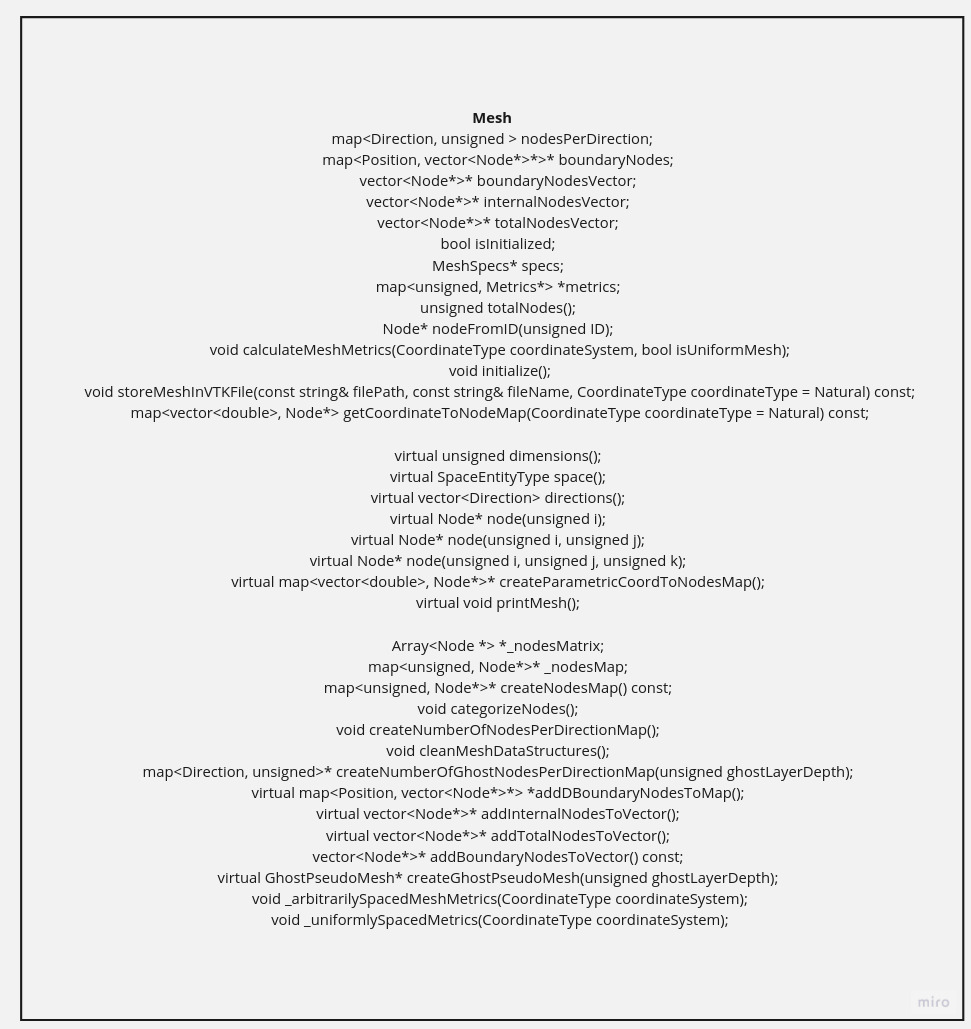
\includegraphics[height=1.0\textheight, width=1.05\textwidth, keepaspectratio]{./images/mesh.jpg}
		\caption{UML Diagram of the Mesh class}
		\label{fig:UML_mesh}
	\end{figure}

	\newpage
	
	\subsubsection{Mesh Generation - Initialization}

		

	The \texttt{MeshFactory} class is responsible for creating and configuring a mesh.
		
\begin{itemize}

	\item When a \texttt{MeshFactory} object is instantiated, it takes in a \texttt{MeshSpecs} object which contains details such as the number of nodes in each direction, the template step size in all Directions as well as the rotation and shear angles for the template mesh.
	
	\item With the \texttt{MeshSpecs} object, the \texttt{MeshFactory} initializes the mesh by invoking the \newline \texttt{\_initiateRegularMesh()} method. This method determines the type of the mesh (1D, 2D, or 3D) based on the number of nodes per direction, and creates a corresponding \texttt{Mesh} object.
	
	
	
	\item The \texttt{NodeFactory} class, which resides in the \texttt{StructuredMeshGenerator} namespace, is responsible for allocating the \texttt{Node*} objects and storing them in an \texttt{Array$<$\texttt{Node}*$>$*}. It also gives the nodes IDs that ascend from Left to Right, Bottom to Top, Back to Front.
	
	\item The parametric and template coordinate vectors are calculated and added to the \texttt{PositionVectors} . by invoking the \texttt{\_assignCoordinates()} method. The appropriate rotation and shear transformations are applied at the parametric coordinates Depending on the type of space entity, it calls one of the methods \texttt{\_assign1DCoordinates()}, \texttt{\_assign2DCoordinates()}, or \texttt{\_assign3DCoordinates()}.
	
	
	\item After assigning the coordinates, \texttt{MeshFactory} calculates the mesh metrics and uses them to compute the PDE properties, which are then stored in \texttt{pdePropertiesFromMetrics}.
	\item Finally, the \texttt{MeshFactory} constructs a \texttt{DomainBoundaryFactory} object for the mesh.
	
	\item After assigning the coordinates, \texttt{MeshFactory} calculates the mesh metrics at each node and uses them to compute the PDE properties, which are then stored in \textit{pdePropertiesFromMetrics}.

\end{itemize}

	
	\subsubsection{Mesh Generation - Metric Tensors Calculation}
	The calculation of the metrics are performed by the \texttt{calculateMetrics} function. The input argument allows for calculation on the template or natural coordinates (only after solution). The process is summurized as follows:
	\begin{itemize}
		\item The function first checks whether the mesh has been initialized. If not, it raises a runtime error. If the mesh is initialized, it proceeds by creating a map to store the mesh metrics.
		
		\item A \texttt{FiniteDifferenceSchemeBuilder} object is created. This object provides access to utility functions needed to construct the finite difference scheme. The function also generates a \texttt{GhostPseudoMesh}, which is an auxiliary mesh that includes additional layers of ghost nodes, facilitating calculations at the boundary. The ghost nodes are initialized in the same way as the rest of the nodes by giving them coordinates that match the template.
		
		\item The function iterates over each node in the mesh. For each node, it generates an \newline \texttt{IsoParametricNodeGraph} object. This object represents the neighbourhood of the node in the mesh, including the number of ghost nodes and diagonal neighbours. 
		
		\item For each node, the function initializes a \texttt{Metrics} object to store the computed metrics. It obtains colinear nodal coordinates for both the parametric and template coordinate systems.
		
		\item The function enters a loop that traverses all spatial directions (I). For each direction, it computes the covariant and contravariant base vectors. These vectors represent the derivatives of real space coordinates with respect to curvilinear coordinates, and vice versa. The function calculates these vectors using appropriate weights and stores them in the \texttt{Metrics} object for the node. The weight calculation can be performed on uniform and non-uniform grids.
		
		\item After processing each direction, the function calculates the covariant and contravariant tensors. These tensors represent the metric tensors in covariant and contravariant forms, respectively. It then adds the \texttt{Metrics} object to the \texttt{metrics} map.
		
		\item Deallocate Memory
	\end{itemize}

	\subsubsection{Mesh Generation - Poisson PDE Equation Solution}
	
	 In the case of Structured Mesh Generation the \texttt{MathematicalProblem} the unknown quantities are the natural coordinates of the internal nodes and they are calculated by solving Laplace or Poison PDE in the parametric space. The numerical simulation is orchestrated by the \texttt{MeshFactory::buildMesh} function : 
 	\begin{itemize}
 		\item The \texttt{MathematicalProblem} is defined as follows :
 			\begin{itemize}
 				\item The contravariant metric tensor components of each node will be imposed as \newline \texttt{SecondOrderLinearPDEProperties}
 				\item The boundary shape is defined by the \texttt{DomainBoundaryFactory} class. The value of the Natural coordinates at the boundaries will act as Dirichlet conditions for the Fixed DOF during the simulation. The available boundary shapes are: 
 			\begin{itemize}
 				\item \texttt{parallelogram} : Parallelogram with input step size, rotation and shear angles.
 				\item \texttt{ellipse} : Ellipse with input a, b.
 				\item \texttt{annulus} : Annulus / Ampitheatre with input inner and outer radii as well as start and end corners
 				\item \texttt{cavityBot} : Parallelogram with input step size, and half-circle cavity on the Bottom boundary.
 				\item \texttt{gasTankHorizontal} : Parallelogram with input step size, and half-circle cavities on the Right and Left Boundaries
 				\item \texttt{sinusRiver} : Top and Bottom boundaries are shapes as sinus curves with the same input A and $\omega$ varying 	by an input distance
 			\end{itemize}
 	\end{itemize}	
 			\item The analysis is performed on the parametric space so all the information regarding the nodal coorinates is provided in the initialize \texttt{Mesh}
 			
 			\item The \texttt{buildMesh} function checks if the boundary conditions have been initialized, creates a \texttt{SteadyStateMathematicalProblem} object which includes the PDE, the boundary conditions, and the DOF, and sets up a solver for this mathematical problem. \newline A \texttt{SteadyStateFiniteDifferenceAnalysis} object is then created. The constructor takes the aformentioned \texttt{SteadyStateMathematicalProblem}, \texttt{Mesh} and user defined \texttt{Solver}, \texttt{SchemeSpecs}, and Parametric coordinate system as input.
 		\end{itemize}
 	
 	
 	The class constructor accepts several pointers to objects including AnalysisDegreesOfFreedom, Mesh, MathematicalProblem, FDSchemeSpecs, and a CoordinateType enum. The constructor subsequently initializes a number of member variables and data structures, including the right-hand side vector, the system matrix, and a map that correlates parametric coordinates with their corresponding nodes in the mesh. Memory management is facilitated by the class destructor, which deletes the linearSystem instance and sets the _mesh pointer to null.
 	
 	The core functionality of this class is embodied in the createLinearSystem() method. This function is responsible for assembling the linear system by iterating over all the free degrees of freedom in the system. For each degree of freedom, a finite difference scheme is calculated based on the problem's specifications, including the order of error for each derivative. The scheme takes into account the neighboring nodes of each degree of freedom, and incorporates the boundary conditions accordingly. Once the coefficients have been calculated, they are incorporated into the system matrix, and the right-hand side vector is updated. The method also records and reports the duration of the system assembly process, providing valuable insights into the performance of the operation.
 	
 	In addition to the principal method, the class comprises several helper methods such as _initiatePositionsAndPointsMap, _getQualifiedFromAvailable, and _getPDECoefficient. These methods provide additional functionality, including the initialization of complex data structures, filtering available positions based on a set of criteria, and retrieving specific coefficients associated with the partial differential equation at a particular node, given the derivative order and direction.	
	
	
	

\end{document}
